\section{Electricity Spot Price Model}
\label{sec:model}
Spot prices demonstrate several features which will need to be included in the model. Specifically, `high volatility, mean-reversion, seasonality, and frequent extreme jumps' \citep{huisman_mahieu_2003}. Mean reversion comes from the existence of a long-term equilibrium which fluctuations return to \citep[p.~26]{pilipovic_2007}. Seasonality is caused by a fundamental change in the equilibrium price caused by heating/cooling demand in the Winter/Summer months \citep[p.~30-31]{pilipovic_2007}. High volatility and price spikes are caused by fluctuations in demand combined with low elasticity of supply since electricity cannot be readily stored \citep[p.~26]{pilipovic_2007}. To account for these features, \cite{huisman_mahieu_2003} proposes the following regime-switching model.

\subsection{Model Specification}
\label{subsec:model-spec}

Let $s(t)$ denote the natural log of the spot price on day $t$ where $t \in \mathbb{Z}_{>0}$.
Then, $s(t)$ is modelled as the sum of a deterministic component $f(t)$ and stochastic component $x(t)$. The deterministic component is given as
\begin{equation}
    f(t) = \mu_0 + \beta_1 D_1(t) + \beta_2 D_2(t)
\end{equation}
where $\mu_1$, $\beta_1$ and $\beta_2$ are parameters in $\mathbb{R}$ and $D_1(t)$ and $D_2(t)$ are dummy variables representing whether day $t$ is a Saturday or Sunday respectively. This accounts for an intraweek demand profile with lower prices during weekends.

The stochastic component is where the regimes come in. The model in \cite{huisman_mahieu_2003} includes three regimes. A regime for normal price levels (regime $0$), a regime for a price spike (regime $1$) and a regime for reverting after a price spike (regime $-1$). Regimes $0$ and $-1$ are specified the same. The inclusion of regime $-1$ allows for proper specification of the mean reversion component. That is, there may be a stronger reverting process after a spike compared to during regime 0 \citep{huisman_mahieu_2003}. To move between regimes, a Markov process on the state space $\{0, +1, -1\}$ with transition diagram given in Figure~\ref{fig:std}, is used.

\subfile{transitiondiagram}

The model starts in regime $0$ (default price levels), then with some probability $1-p$ it moves to regime $1$ (the price spike regime). The day after entering regime $1$ it enters regime $-1$ (the reverting regime). Then, the day after that, it returns to regime $0$.

The regimes are specified in terms of the day-on-day change in the stochastic component $\dif{x(t)} := x(t) - x(t-1)$ with $x(1)=0$. Let $(\epsilon_t)$ be a sequence of independent standard Normal random variables. For normal price levels (regime $0$) model
\begin{equation}
    \dif{x(t)} = -\alpha_0 x(t-1) + \sigma_0 \epsilon_t
\end{equation}
where $\alpha_0 \in (0,1)$ and $\sigma_0 \in (0, \infty)$ are parameters. Parameter $\alpha_0$ specifies the level of mean reversion. That is, the greater $\alpha_0$ is, the quicker any fluctuations away from the deterministic component will be restored.

The reverting regime (regime -1) is modelled exactly the same. Model
\begin{equation}
    \dif{x(t)} = -\alpha_{-1} x(t-1) + \sigma_{-1} \epsilon_t
\end{equation}
where $\alpha_{-1} \in (0,1)$ and $\sigma_{-1} \in (0, \infty)$ are parameters.
Finally for the spike regime (regime $1$) a Normally distributed price spike is introduced as
\begin{equation}
    \label{eqn:spike}
    \dif{x(t)} = \mu_1 + \sigma_{1} \epsilon_t
\end{equation}
where $\mu_1 \in \mathbb{R}$ and $\sigma_1 \in (0, \infty)$ are parameters.

This completes the specification of the model. The next section will look at how the constrained parameters in the model can be handled.

\subsection{Constrained Parameters}
\label{subsec:constr-par}
In the model, there are several constrained parameters. These will be handled by introducing unconstrained transformed parameters. Consider the functions $f(x) = e^x$ and $g(x) = \frac{e^x}{1 - e^x}$. Both functions are defined on $\mathbb{R}$ and are invertible. Further, the image of $f$ is $(0, \infty)$ and the image of $g$ is $(0,1)$. Thus, for the parameters constrained to $(0, \infty)$, unconstrained parameters $\tau_{\sigma_i}$ where $\sigma_i = f(\tau_{\sigma_i})$ for $i=0, 1, -1$ can be used. Similarly, unconstrained parameters $\tau_p$ and $\tau_{\alpha_j}$ where $p = g(\tau_p)$ and $\alpha_j = g(\tau_{\alpha_j})$ for $j=0,-1$ can be used for the parameters constrained to $(0,1)$. Now, the task is to infer unconstrained parameters: $\mu_0, \beta_1, \beta_2, \tau_{\alpha_0}, \tau_{\sigma_0}, \mu_1, \tau_{\sigma_1}, \tau_{\alpha_{-1}}, \tau_{\sigma_{-1}}$ and $\tau_p$.

Before introducing Synthetic Likelihoods, it is beneficial to look at some example trajectories to better understand of how varying certain parameters affect the model.

\subsection{Example Trajectories}

As will be seen in Sections~\ref{sec:sl} and~\ref{sec:fitting}, the process of choosing statistics for Synthetic Likelihoods is a creative and visual process that requires an understanding of how the model parameters affect the resulting trajectory. This section will provide intuition for the mean reversion parameter, $\alpha_0$, as well as the spike parameters, $\mu_1$ and $p$. The fitted parameters from \cite{huisman_mahieu_2003} for the UK Power Market (Table~\ref{tab:uk-val}) will be used as defaults; values differing from Table~\ref{tab:uk-val} will be noted.

\begin{table}[H]
\caption{Fitted Parameter Values for UK
\label{tab:uk-val}
Telerate Market \citep{huisman_mahieu_2003}}
\begin{tabular}{@{}lllllllllll@{}}
\toprule
\textbf{Parameter}: & $\mu_0$ & $\beta_1$ & $\beta_2$ & $\alpha_0$ & $\sigma_0$ & $\mu_1$ & $\sigma_1$ & $\alpha_{-1}$ & $\sigma_{-1}$ & $p$  \\
\midrule
\textbf{Value}: & $2.852$   & $-0.089$    & $-0.192$    & $0.112$      & $0.144$      & $0.103$   & $0.542$      & $0.313$         & $0.453$         & $0.95$ \\
\bottomrule
\end{tabular}
\end{table}

First, consider the mean reversion parameter $\alpha_0$. In Figure~\ref{fig:mr_param} it can be seen that setting $\alpha_0 = 0$ makes the resulting trajectory smoother and there appears to be a downwards trend that would have been rectified by introducing some mean-reversion. When it comes to using Synthetic Likelihoods, as will be seen in Section~\ref{sec:sl}, statistics need to be chosen that represent the dynamics of the model. For example, the plots in Figure~\ref{fig:mr_param} suggest different relationships between $s(t)$ and $s(t-1)$. Thus, autocorrelation coefficients may be useful statistics to include.

\begin{figure}[H]
    \centering
    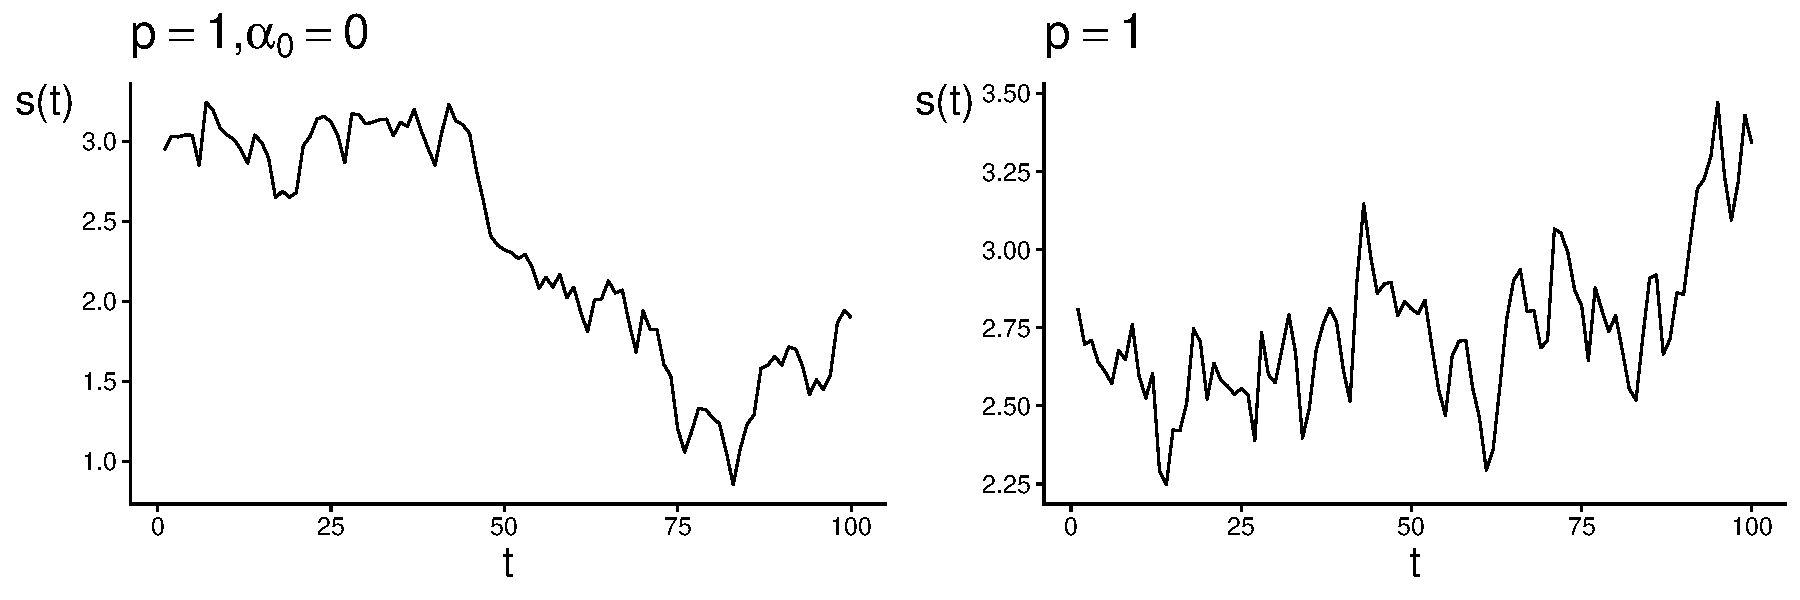
\includegraphics[width=12cm]{images/model/mean_reversion_example.pdf}
    \caption{Understanding the Mean Reversion Parameter}
    \label{fig:mr_param}
\end{figure}

Moving to the spike parameters. Figure~\ref{fig:spike_param} shows graphs with different parameters for $\mu_1$ and $p$. Clearly, $\mu_1$ controls the average height of the spikes and $p$ the frequency of spikes. Statistics that capture the effects of these parameters will be presented in Section~\ref{subsec:full-stats}.


\begin{figure}[H]
    \centering
    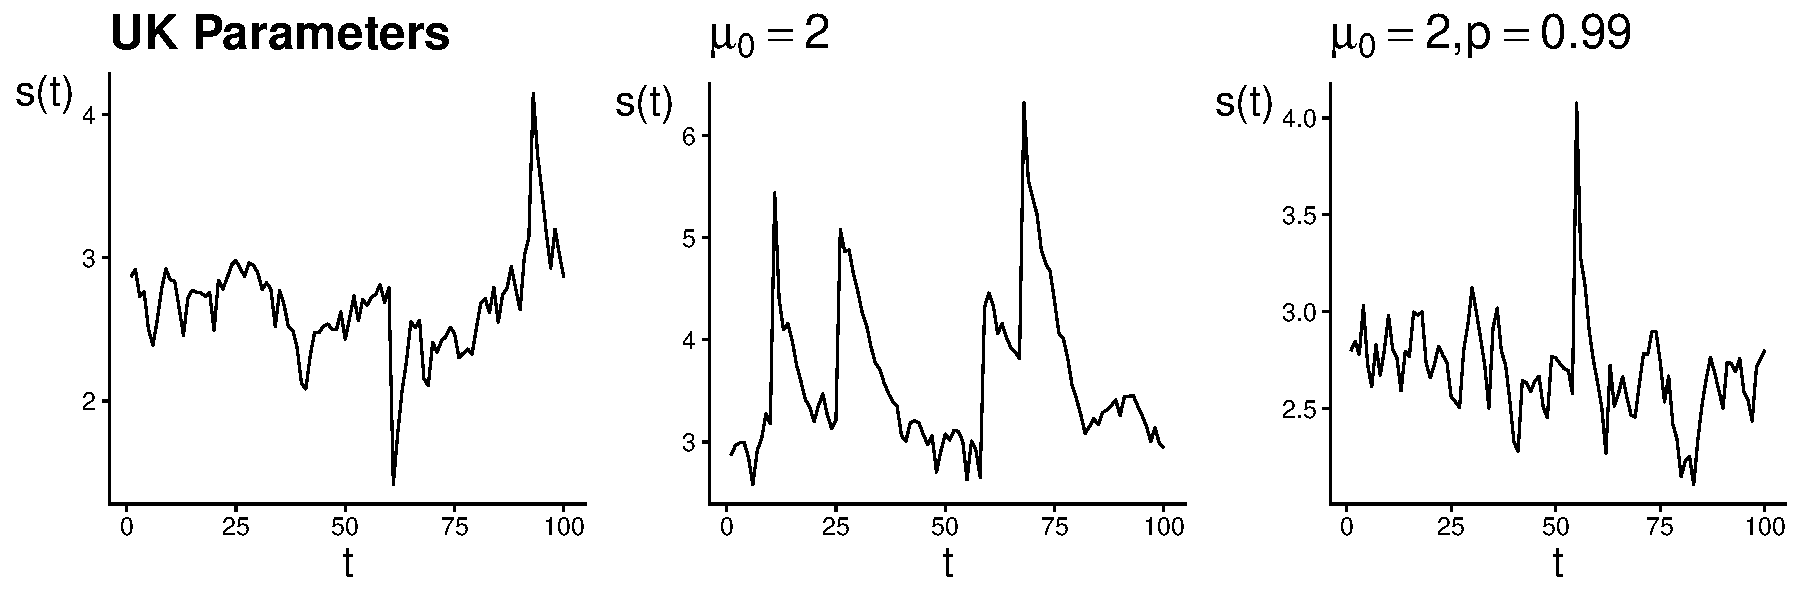
\includegraphics[width=12cm]{images/model/spike_example.pdf}
    \caption{Understanding the Spike Parameters}
    \label{fig:spike_param}
\end{figure}

Now that a model that can capture the nuance of electricity prices has been specified, the next section will introduce Synthetic Likelihoods. From this point forward, the model put forward in this section will be referred to as Model $\mathcal{A}$.